\begin{figure}[h]
    \begin{subfigure}[b]{0.5\textwidth}
        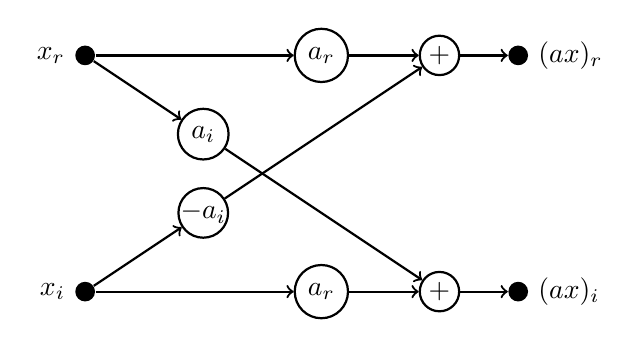
\begin{tikzpicture}[
                dot/.style = {circle, fill, inner sep = 0mm, minimum size = 2.5mm},
                op/.style = {draw, thick, circle, inner sep = 0mm, minimum size = 5mm},
                func/.style = {draw, thick, circle, inner sep = 1mm},
                arr/.style = {draw, thick, ->},
            ]
            \node (XR) [dot, label=left:$x_r$] at (0,3){};
            \node (XI) [dot, label=left:$x_i$] at (0,0){};
            \node (AXR) [dot, label=right:$(ax)_r$] at (5.5,3){};
            \node (AXI) [dot, label=right:$(ax)_i$] at (5.5,0){};

            \node (P1) [op] at (4.5, 3) {+};
            \node (P2) [op] at (4.5, 0) {+};
            \node (AR1) [func] at (3.0, 3) {$a_r$};
            \node (AR2) [func] at (3.0, 0) {$a_r$};

            \node (AI1) [func] at (1.5, 2) {$a_i$};
            \node (AI2) [op] at (1.5, 1) {$-a_i$};

            \path[arr] (XR) -- (AR1);
            \path[arr] (AR1) -- (P1);
            \path[arr] (P1) -- (AXR);

            \path[arr] (XI) -- (AR2);
            \path[arr] (AR2) -- (P2);
            \path[arr] (P2) -- (AXI);

            \path[arr] (XR) -- (AI1);
            \path[arr] (AI1) -- (P2);

            \path[arr] (XI) -- (AI2);
            \path[arr] (AI2) -- (P1);
        \end{tikzpicture}
        \caption{Butterfly structure.\label{fig:complexmula}}
    \end{subfigure}
    \begin{subfigure}[b]{0.5\textwidth}
        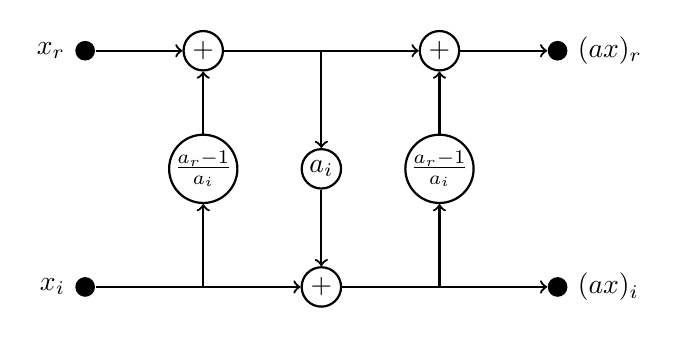
\begin{tikzpicture}[
                dot/.style = {circle, fill, inner sep = 0mm, minimum size = 2.5mm},
                op/.style = {draw, thick, circle, inner sep = 0mm, minimum size = 5mm},
                func/.style = {draw, thick, circle, inner sep = 1mm},
                arr/.style = {draw, thick, ->},
            ]
            \node (xr) [dot, label=left:$x_r$] at (0,3){};
            \node (xi) [dot, label=left:$x_i$] at (0,0){};
            \node (axr) [dot, label=right:$(ax)_r$] at (6,3){};
            \node (axi) [dot, label=right:$(ax)_i$] at (6,0){};

            \node (one) [op] at (1.5, 1.5) {$\frac{a_r - 1}{a_i}$};
            \node (two) [op] at (3, 1.5) {$a_i$};
            \node (three) [op] at (4.5, 1.5) {$\frac{a_r - 1}{a_i}$};

            \node (p1) [op] at (1.5, 3){+};
            \node (p2) [op] at (3, 0){+};
            \node (p3) [op] at (4.5, 3){+};

            \path[arr] (xr) -- (p1);
            \path[arr] (p1) -- (p3);
            \path[arr] (p3) -- (axr);

            \path[arr] (xi) -- (p2);
            \path[arr] (p2) -- (axi);

            \path[arr] (1.5, 0) -- (one);
            \path[arr] (one) -- (p1);

            \path[arr] (3, 3) -- (two);
            \path[arr] (two) -- (p2);

            \path[arr] (4.5, 0) -- (three);
            \path[arr] (three) -- (p3);
        \end{tikzpicture}
        \caption{Alternative lifting scheme.\label{fig:complexmulb}}
    \end{subfigure}
    \begin{subfigure}[b]{0.5\textwidth}
        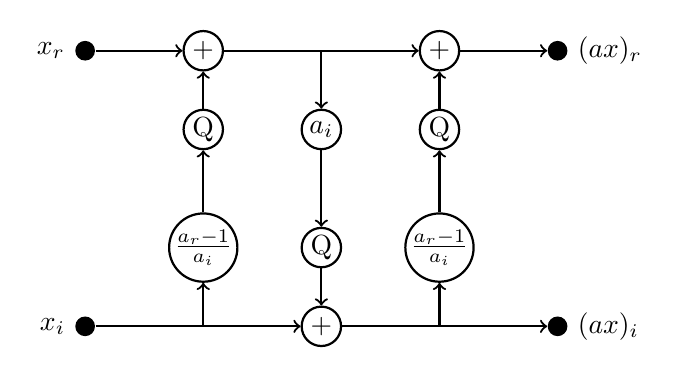
\begin{tikzpicture}[
                dot/.style = {circle, fill, inner sep = 0mm, minimum size = 2.5mm},
                op/.style = {draw, thick, circle, inner sep = 0mm, minimum size = 5mm},
                func/.style = {draw, thick, circle, inner sep = 1mm},
                arr/.style = {draw, thick, ->},
            ]
            \node (xr) [dot, label=left:$x_r$] at (0,3.5){};
            \node (xi) [dot, label=left:$x_i$] at (0,0){};
            \node (axr) [dot, label=right:$(ax)_r$] at (6,3.5){};
            \node (axi) [dot, label=right:$(ax)_i$] at (6,0){};

            \node (one) [op] at (1.5, 1) {$\frac{a_r - 1}{a_i}$};
            \node (two) [op] at (3, 2.5) {$a_i$};
            \node (three) [op] at (4.5, 1) {$\frac{a_r - 1}{a_i}$};

            \node (q1) [op] at (1.5, 2.5){Q};
            \node (q2) [op] at (3, 1){Q};
            \node (q3) [op] at (4.5, 2.5){Q};

            \node (p1) [op] at (1.5, 3.5){+};
            \node (p2) [op] at (3, 0){+};
            \node (p3) [op] at (4.5, 3.5){+};

            \path[arr] (xr) -- (p1);
            \path[arr] (p1) -- (p3);
            \path[arr] (p3) -- (axr);

            \path[arr] (xi) -- (p2);
            \path[arr] (p2) -- (axi);

            \path[arr] (1.5, 0) -- (one);
            \path[arr] (one) -- (q1);
            \path[arr] (q1) -- (p1);

            \path[arr] (3, 3.5) -- (two);
            \path[arr] (two) -- (q2);
            \path[arr] (q2) -- (p2);

            \path[arr] (4.5, 0) -- (three);
            \path[arr] (three) -- (q3);
            \path[arr] (q3) -- (p3);
        \end{tikzpicture}
        \caption{Lifting scheme with quantization.\label{fig:complexmulc}}
    \end{subfigure}
    \caption{Datapaths for complex multiplication.\label{fig:complexmul}}
\end{figure}
